\documentclass[11pt]{book}
\usepackage{fullpage, amsfonts}
\usepackage{varwidth}
\usepackage{float}
\usepackage{bez123}
\usepackage{amsmath}
\usepackage{amssymb}
\usepackage{color}
\usepackage{xcolor,graphicx}
\usepackage{tikz}
\usetikzlibrary{shapes,arrows,decorations.pathmorphing,backgrounds,fit}


\newcommand{\gnote}[1]{{{\sf (Gilad's Note:} {\sl{#1}} {\sf EON)}}}

\newtheorem{thm}{Theorem.}[section]      % A counter for Theorems etc
\newcommand{\BT}{\begin{thm}}   \newcommand{\ET}{\end{thm}}
\newtheorem{dfn}[thm]{Definition.}      %
\newcommand{\BD}{\begin{dfn}}   \newcommand{\ED}{\end{dfn}}
\newtheorem{corr}[thm]{Corollary.}      %
\newcommand{\BCR}{\begin{corr}} \newcommand{\ECR}{\end{corr}}
\newtheorem{lem}[thm]{Lemma.}
\newcommand{\BL}{\begin{lem}}   \newcommand{\EL}{\end{lem}}
\newtheorem{prop}[thm]{Proposition.}
\newcommand{\BP}{\begin{prop}}   \newcommand{\EP}{\end{prop}}
\newtheorem{clm}[thm]{Claim.}            %
\newcommand{\BCM}{\begin{clm}}   \newcommand{\ECM}{\end{clm}}
\newtheorem{fact}[thm]{Fact.}            %
\newcommand{\BF}{\begin{fact}}   \newcommand{\EF}{\end{fact}}
\newtheorem{nota}[thm]{Notation.}            %
\newcommand{\BN}{\begin{nota}}   \newcommand{\EN}{\end{nota}}
\newtheorem{property}[thm]{Property.}
\newcommand{\BPRO}{\begin{property}} \newcommand{\EPRO}{\end{property}}
\newtheorem{algorithm}[thm]{Algorithm.}            %
\newcommand{\BAL}{\begin{algorithm}}   \newcommand{\EAL}{\end{algorithm}}

\def\blackslug
{\hbox{\hskip 1pt\vrule width 8pt height 8pt depth 1.5pt\hskip 1pt}}
\def\qed{\quad\blackslug\lower 8.5pt\null\par}
\def\qqed{$\Box$}

\newcommand{\BPR}{\begin{myprot}}   \newcommand{\EPR}{\end{myprot}}
\newenvironment{proof}{\noindent{\bf Proof.~~}}{\qed}
\newcommand{\BPF}{\begin{proof}} \newcommand {\EPF}{\hfill\end{proof}}
\newenvironment{proofsketch}{\noindent{\bf Proof Sketch.~~}}{\qed}
\newcommand{\BPFS}{\begin{proofsketch}} \newcommand {\EPFS}{\hfill\end{proofsketch}}


\makeatletter
%%%%%%%%%%%%%%%%%%%%%%%%%%%%%%% User specified LaTeX commands.
\author{notes by\\ G.~Hoch \&~A.~Aped}
\title{\Huge \textbf{Advanced Data Structures}\\ 
\LARGE Based on the lectures of Prof. Moshe Lewinstein}
%\usepackage[dvipdf]{graphicx}
%\usepackage{bez123}
%\usepackage{amsmath}

%\makeatother

%\usepackage{babel}

\begin{document}
\maketitle
\tableofcontents
\newpage

\chapter{The Dictionary Problem}
Given a ``world'' $U$ such that:
\[U:=\{0,1,\ldots{},u-1\}\]
we want to store a sub-group $S\subseteq U$ such that $|S|=n$ \\*
and we want to support several queries over $S$:
\flushleft
\begin{enumerate}
\item Existence:
\begin{itemize}
\item \textbf{input:} $x\in U$
\item \textbf{output:} $1$ if $x\in S$, $0$ otherwise.
\end{itemize}
\item Successor
\begin{itemize}
\item \textbf{input:} $x\in U$
\item \textbf{output:} $y|y=min\{z\in S|x\le z\}$
\end{itemize}
\item Predecessor
\begin{itemize}
\item \textbf{input:} $x\in U$
\item \textbf{output:} $y|y=max\{z\in S|x\ge z\}$
\end{itemize}
\item Insert
\begin{itemize}
\item \textbf{input:} $x\in U$
\item \textbf{output:} $S\gets S\bigcup \{x\}$
\end{itemize}
\item Delete
\begin{itemize}
\item \textbf{input:} $x\in U$
\item \textbf{output:} $S\gets S \backslash \{x\}$
\end{itemize}
\end{enumerate}
\newpage

%\section{Hashing}
We will try to deal with the existence problem:
\section{Universal Hashing, Perfect Hashing \& FKS}
On the following proposals, we will try to answer the questions:
\flushleft
\begin{enumerate}
\item How long does the query take?
\item What is the size of the data structure for $S$?
\item How long does it take to build this data structure?
\item Does the data structure support changes (insert\slash delete)?
\end{enumerate}
\medskip
Possible solutions:
\BP
\label{prop:FKS.I}
(for fast queries)\\*
we will store an array $A$ the size of $u$, such that $A[i]$ \linebreak[3] 
(where $0\le i\le u-1$) contain $true \iff i\in S$ \\*
\textbf{Space:} $O(u)$\\*
\textbf{Time:} $O(1)$\\*
\EP
\BP
(for space efficiency)\\*
a sorted array for $S$, for every query we can use binary search\\*
\textbf{Space:} $O(n)$\\*
\textbf{Time:} $O(log(n))$\\*
\EP
\BP
(for both space \& time efficiency)\\*
Hash function:\\
%%%%%%%%%%%%%%%%%%%
% PICTURE 1 BEGIN %
%%%%%%%%%%%%%%%%%%%
\setlength{\unitlength}{10mm}
\begin{picture}(4,6)
\linethickness{0.2mm}
\put(3,0){\line(0,1){6}}
\put(4,0){\line(0,1){6}}
\put(3,0){\line(1,0){1}}
\put(3,1){\line(1,0){1}}
\put(3,4){\line(1,0){1}}
\put(3,5){\line(1,0){1}}
\put(3,6){\line(1,0){1}}

\put(1,3){$h:U $}
\put(2,3){$\longrightarrow $}

\put(3.4,5.4){$0$}
\put(3.4,4.4){$1$}
\put(3.085,0.4){$g-1$}
\put(3.4,2.5){\vdots}

\end{picture}  \\*
%%%%%%%%%%%%%%%%%
% PICTURE 1 END %
%%%%%%%%%%%%%%%%%
we would want to ensure that $g=O(n)$, one way to ensure that, 
is to use chaining, but then, worst case scenario, 
if we have a lot of collisions, queries will take longer than $O(1)$. 
another option is to choose a "good" function $h:U\to[c\cdot n]$. 
if we take a random function, then the number of collisions will be $O(1)$, 
but it is highly unlikely to find a compact representation for a random function. 
that is, the only way to represent the function, is with a table the of size $u$: \\*
\medskip
%%%%%%%%%%%%%%%%%%%
% PICTURE 2 BEGIN %
%%%%%%%%%%%%%%%%%%%
\setlength{\unitlength}{10mm}
\begin{picture}(5,7)
\linethickness{0.2mm}

\put(1,0){\line(0,1){7}}
\put(2,0){\line(0,1){7}}
\put(4,1.5){\line(0,1){4}}
\put(5,1.5){\line(0,1){4}}

\put(1,7){\line(1,0){1}}
\put(1,6){\line(1,0){1}}
\put(1,1){\line(1,0){1}}
\put(1,0){\line(1,0){1}}

\put(4,5.5){\line(1,0){1}}
\put(4,4.5){\line(1,0){1}}
\put(4,2.5){\line(1,0){1}}
\put(4,1.5){\line(1,0){1}}

\put(1.4,6.4){$0$}
\put(1.08,0.4){$u-1$}
\put(1.4,3.25){\vdots}

\put(4.3,4.9){$s_1$}
\put(4.3,1.9){$s_n$}
\put(4.4,3.25){\vdots}

\cbezier(2,2.5)(2.75,2.5)(3.25,4)(4,4)
\cbezier(2,0.5)(2.75,0.5)(3.25,5)(4,5)
\cbezier(2,6.5)(2.75,6.5)(3.25,3)(4,3)
\cbezier(2,5.5)(2.75,5.5)(3.25,2)(4,2)
\end{picture}  \\*
%%%%%%%%%%%%%%%%%
% PICTURE 2 END %
%%%%%%%%%%%%%%%%%
so it didn't save us space, 
and we are better off with the 
naieve solution suggested in Proposition~\ref{prop:FKS.I} 
(a boolean array the size of $u$).
\EP
\subsubsection{Universal Hashing}
%\underline{\textbf{\emph{Universal Hashing}}}\\*
\BD
a family $\mathcal{H}$ of hash functions $h:U\to [m]
      \textcolor[rgb]{1,0,0}{
	\footnotemark}
$ is called {\sf universaly weak}, 
if for some $x,y\in U$ and for every $h\in \mathcal{H}$:
\footnotetext{$[m]=\{0,\ldots{},m-1\}$}
$$Pr\bigg[ h(x)=h(y)\bigg]\le \frac{1}{m}$$
\ED
assuming we are using a universaly weak function $h$, 
what would be the expected number of collisions?\\
$$I_x(y)=\left\{
	  \begin{array}{rl}
	    1 & h(x)=h(y)\\
	    0 & otherwise
	  \end{array} 
	\right.$$
well, the number of collisions on $h(x)$ is:
$$\sum_{y\in S}{I_x(y)}$$
so the expected number of collisions is:
$$ E\Big(\sum_{y\in S}{I_x(y)}\Big)=
    \sum_{y\in S}{E\Big(I_x(y)\Big)}=
    \sum_{y\in S}{Pr\Big[h(x)=h(y)\Big]}=
    1+\sum_{y\ne x}{Pr\Big[h(x)=h(y)\Big]}\le 
    1+(n-1)\frac{1}{m}$$
So, if we choose $m=n$, we will get that the 
expected number of collisions\nolinebreak[4] $\le 1+1=2$\\
OK, so how can we find such functions?\\*
$h_{a,b}(x)=((a\cdot x+b) \bmod p)\bmod m$, where $p$ is prime, 
and $m<p$, also $a,b\in \{0,\dots{},p-1\}, a\ne 0$, 
$\mathcal{H}_{p}=\{h_{a,b}|0<a\le p-1,0\le b\le p-1\}$
\BCM
$\mathcal{H}_{p}$ is universaly weak.
\ECM
\BPF
Omitted. Can be found in~\cite{Cormen}.
\EPF
\BD
a hash function is {\sf perfect} for $S\subseteq U$ 
if $\forall x,y\in S, x\ne y\Longrightarrow h(x)\ne h(y)$
\ED
We will take a universal family $\mathcal{H}_m$, such that $m=n^2$, 
and pick $h\in \mathcal{H}_m$ at random.\\*
$ \mathcal{H}_m=
    \textcolor[rgb]{1,0,0}{
      \footnotemark}
  \{h_1,\dots{},h_{m^2}\}=\{h_1,\dots{},h_{n^4}\}$, $S=\{x_1,\dots{},x_n\}$\\*
\footnotetext{there are $m$ possibilities to choose the coefficient $a$, 
		and $m$ possibilities to choose $b$, so overall, 
		the function family $\mathcal{H}_m$ contain $m\cdot m$ distinct functions.}
$$\text{\#collisions}=\sum_{
			\substack{x\ne y\\* x,y\in S}
			   }
		      I_{x}(y)
			\textcolor[rgb]{1,0,0}{\footnotemark}
\footnotetext{where $I_{x}(y)$ is same as before: $I_x(y)=
			    \left\{
			      \begin{array}{rl}
				1 & h(x)=h(y)\\
				0 & otherwise
			      \end{array} 
			    \right.$}$$
$$E\Big(\sum_{
	  \substack{x\ne y\\* x,y\in S}}
	I_{x}(y)\Big)=
	\sum_{
	  \substack{x\ne y\\* x,y\in S}}
	E\Big(I_{x}(y)\Big)=
	\sum_{
	  \substack{x\ne y\\* x,y\in S}}
	Pr\Big[h(x)=h(y)\Big]\le 
	\binom{n}{2}\cdot{}\frac{1}{m}=
	\frac{n(n-1)}{2}\cdot{}\frac{1}{n^2}\le 
	\frac{1}{2}$$
$$\Longrightarrow 
  Pr\Big[\text{there's a collision}\Big]=
    \textcolor[rgb]{1,0,0}{\footnotemark}
\footnotetext{\textbf{reminder.} Markov's inequality: $Pr\big[X\ge t\big]\le \frac{E(X)}{t}$}
  Pr\Big[X
    \textcolor[rgb]{1,0,0}{\footnotemark}
\footnotetext{$X$ is the random variable that stands for the number of collisions.}
  \ge 1\Big]\le \frac{ \frac{1}{2}}{1}=\frac{1}{2}$$
So actually, not only the expectation for a collision $\le \frac{1}{2}$, 
the chance that there will even be a collision is equal to $\frac{1}{2}$. 
checking for collisions = building the table: $h(x_1),h(x_2),\dots{},h(x_n)$\\
an algorithm to build a perfect hash function, when $m=n^2$:
\BAL
\item[1.] take the universal family $\mathcal{H}_{n^2}$.
\item[2.] choose $h\in \mathcal{H}_{n^2}$ at random.
\begin{itemize}
 \item[2.1.] if $h$ is not perfect for $S$, go back to 2.
\end{itemize}
\EAL
%\begin{equation*}
\begin{align*}
E\Big(\text{the algorithm running time}\Big) &=
  \sum_{i=1}^{\infty}n\cdot{}Pr\Big[\text{the algorithm ran for $i$ iterations}\Big]\nonumber \\
  &= \sum_{i=1}^{\infty}n\cdot{}\frac{1}{2^i}=
  n\cdot{}\sum_{i=1}^{\infty}\frac{1}{2^i}=
  2n\nonumber
\end{align*}
%\end{equation*}
at the end of the process, we were able to find a perfect hash function for $S$, 
such that the expected time for building the function is $2n (O(n))$, 
and query time is always $O(1)$. the downside of the solution is about the space complexity. 
that's because we pay $m=n^2$ in space for the table, when most of it stays empty.\\
\medskip
\textbf{Space:} $O(n^2)$\\*
\textbf{Query Time:} $O(1)$\\*
\textbf{Build Time:} $E\big(O(n)\big)$\\* 
\newpage
improvment: FKS\textcolor[rgb]{1,0,0}{\footnotemark} method.\\*
\footnotetext{FKS - Michael L. Fredman and
               J{\'a}nos Koml{\'o}s and
               Endre Szemer{\'e}di~\cite{FKS82}}
we will choose $m=n$:
$$E\Big(\text{the number of collisions}\Big)
  \textcolor[rgb]{1,0,0}{\footnotemark}
\le \binom{n}{2}\cdot{}\frac{1}{m}=
\frac{n(n-1)}{2}\cdot{}\frac{1}{n}\le \frac{n}{2}
\footnotetext{according to Markov's inequality theorem:
      $Pr\bigg[X\ge n\bigg]\le \frac{\frac{n}{2}}{n}=\frac{1}{2}$
      , and that's why finding a function $h$ with $n$ collisions at most, 
      would take 2 iterations (in expectation).}$$
and then we can make perfect hashing over the collision groups $S_i$
\medskip
%%%%%%%%%%%%%%%%%%%
% PICTURE 3 BEGIN %
%%%%%%%%%%%%%%%%%%%
\setlength{\unitlength}{10mm}
\begin{picture}(12,8)
\linethickness{0.2mm}
%
\put(1,0){\line(0,1){8}}
\put(2,0){\line(0,1){8}}
\put(9,1.5){\line(0,1){4}}
\put(10,1.5){\line(0,1){4}}
%
\put(1,8){\line(1,0){1}}
\put(1,7){\line(1,0){1}}
\put(1,6){\line(1,0){1}}
\put(1,4){\line(1,0){1}}
\put(1,3){\line(1,0){1}}
\put(1,1){\line(1,0){1}}
\put(1,0){\line(1,0){1}}
%
\put(9,5.5){\line(1,0){1}}
\put(9,4.5){\line(1,0){1}}
\put(9,2.5){\line(1,0){1}}
\put(9,1.5){\line(1,0){1}}
%
\put(1.4,7.4){$0$}
\put(1.4,6.4){$1$}
\put(1.4,3.4){$i$}
\put(1.08,0.4){$n-1$}
\put(1.4,4.75){\vdots}
\put(1.4,1.75){\vdots}
%
\put(4,3){\line(1,0){3}}
\put(4,4){\line(1,0){3}}
\put(4,3){\line(0,1){1}}
\put(7,3){\line(0,1){1}}
%
\put(4.5,3.42){$n_i$ collisions}
%
\put(2,7.5){\vector(1,0){2}}
\put(2,6.5){\vector(1,0){2}}
\put(2,3.5){\vector(1,0){2}}
\put(7,3.5){\vector(1,0){2}}
\put(2,0.5){\vector(1,0){2}}
%
\put(4.25,7.475){\dots{}}
\put(4.25,6.475){\dots{}}
\put(4.25,0.475){\dots{}}
%
\cbezier(10.25,1.5)(10.75,1.5)(10.25,3.5)(10.75,3.5)
\cbezier(10.25,5.5)(10.75,5.5)(10.25,3.5)(10.75,3.5)
%
\put(9.4,4.85){$0$}
\put(9.15,1.85){$n_i^2 $-$1$}
\put(9.4,3.25){\vdots}
%
\put(11,3.42){$n_i^2$}
\end{picture}  \\*
%%%%%%%%%%%%%%%%%
% PICTURE 3 END %
%%%%%%%%%%%%%%%%%
\medskip
$S_i=\{x\in S|h(x)=i\}, |S_i|=n_i$\\*
we will apply perfect hashing for $S_i$, 
so that the ``main'' hash table contains 
only a pointer to a secondary hash table for $S_i$
\BAL
\item[1.] take the universal family $\mathcal{H}_{n}$.
\item[2.] choose $h\in \mathcal{H}_{n}$ at random.
\begin{itemize}
 \item[2.1.] if the number of collisions in $h>n$, go back to 2.
\end{itemize}
\item[3.] create a table for $h:S\to [n]$.
\item[4.] for every index $i$ in the table:
\begin{itemize}
 \item[4.1] choose $h_i\in \mathcal{H}_{n_i^2}$ at random.
 \item[4.2] if $h_i$ is not perfect hash for $S_i$, go back to 5.1.
\end{itemize}
\EAL
\newpage
But, we do have some open questions:\\*
\begin{enumerate}
 \item How much space is required for this data structure?
 \item how long doe's it takes to build it?
\end{enumerate}
%%%%%%%%%%%%%%%%%%%
% PICTURE 4 BEGIN %
%%%%%%%%%%%%%%%%%%%
\setlength{\unitlength}{10mm}
\begin{picture}(9,10)
\linethickness{0.2mm}

\put(2,1){\line(0,1){8}}
\put(3,1){\line(0,1){8}}
\put(6,2.5){\line(0,1){4}}
\put(7,2.5){\line(0,1){4}}

\put(2,9){\line(1,0){1}}
\put(2,8){\line(1,0){1}}
\put(2,6){\line(1,0){1}}
\put(2,5){\line(1,0){1}}
\put(2,2){\line(1,0){1}}
\put(2,1){\line(1,0){1}}

\put(6,6.5){\line(1,0){1}}
\put(6,5.5){\line(1,0){1}}
\put(6,3.5){\line(1,0){1}}
\put(6,2.5){\line(1,0){1}}

\put(2.4,8.4){$0$}
\put(2.4,5.4){$i$}
\put(2.08,1.4){$n-1$}
\put(2.425,6.75){\vdots}
\put(2.425,3.25){\vdots}

\cbezier(7.25,2.5)(7.75,2.5)(7.25,4.5)(7.75,4.5)
\cbezier(7.25,6.5)(7.75,6.5)(7.25,4.5)(7.75,4.5)

\cbezier(1.75,1)(1.25,1)(1.75,5)(1.25,5)
\cbezier(1.75,9)(1.25,9)(1.75,5)(1.25,5)

\put(3,5.5){\line(1,0){0.5}}
\cbezier(3.5,5.5)(4.5,5.5)(4.5,4.5)(5.5,4.5)
\put(5.5,4.5){\vector(1,0){0.5}}

\put(6.4,5.85){$0$}
\put(6.15,2.85){$n_i^2 $-$1$}
\put(6.4,4.25){\vdots}

\put(8,4.42){$n_i^2$}
\put(0.85,4.92){$n$}

\end{picture}
%%%%%%%%%%%%%%%%%
% PICTURE 4 END %
%%%%%%%%%%%%%%%%%

The size of this data structure is: 
$$O\bigg(n+\sum_{i=0}^n{n_i^2}\bigg)=\textcolor[rgb]{1,0,0}{\footnotemark}
O\big(n+\text{(\# collisions)}\big)=
O(n)$$
\footnotetext{when $n_i$ elements, all colliding with each other, 
it means we have $\frac{n_i(n_i-1)}{2}$ collisions, 
and that is why $n_i\le \sqrt{n}$, so $n_i^2\le n$, 
since all the collisions in $S$ are less than $n$, i.e. $\sum_{}n_i \le n \Longrightarrow{}
n=(\sqrt{n})^2\ge \sum_{}n_i^2$}
$\Longrightarrow{}$ the space complexity is\\*
\textbf{Space:} $O(n)$\\*
what about time complexity?\\*
\textbf{Build time:} $O\big(n+\sum{}n_i\big)=O(n)$\textcolor[rgb]{1,0,0}{\footnotemark}
\footnotetext{in expectation}\\*
\textbf{Query time:} $O(1)$\textcolor[rgb]{1,0,0}{\footnotemark}
\footnotetext{Query algorithm:
  \BAL
    \item[1.] search the main table for a pointer to $n_i$, if null return false.
    \item[2.] search $n_i$ for the requested element and return the answer.
  \EAL
  this algorithm works in constant time, and this is why query time is always $O(1)$.
}
\newpage

%\section{Trees \& Tree-like Data structures}
\section{Van-Emde Boas}
\label{subsection:VEB}
\textbf{reminder.} we have a world $U=\{0,\dots{},u-1\}$, and a subset $S\subseteq U$. 
we want to support the actions: \emph{insert,delete,successor,predecessor},
where \emph{successor} \& \emph{predecessor} are defined by:
$$succ(x) = y|y=min\{z\in S|x\le z\}$$
$$pred(x) = y|y=max\{z\in S|x\ge z\}$$
which (simple) data structure can we use to support these actions?\textcolor[rgb]{1,0,0}{\footnotemark}
\footnotetext{the \emph{predecessor} is symetric to the \emph{successor}, so from now on, 
without loss of generality, can talk only on \emph{successor} (\emph{predecessor} will 
be implemented much like \emph{successor}). also, \emph{delete} can be implemented with a 
``flag'' indicating if the element was deleted or not, so we will not mention \emph{delete} either.}
\BP
\label{prop:VEB.I}
we can store $S$'s elements in an array.
\begin{itemize}
 \item[Option 1.] {
  the array will be the size of $|S|$:\\*
  \medskip
  $S=\{x_1,\dots{},x_n\}$

  \medskip
  \begin{picture}(7,1)
   \put(1,0){\line(1,0){6}}
   \put(1,1){\line(1,0){6}}

   \put(1,0){\line(0,1){1}}
   \put(2,0){\line(0,1){1}}
   \put(3,0){\line(0,1){1}}
   \put(6,0){\line(0,1){1}}
   \put(7,0){\line(0,1){1}}

   \put(0,0.4){$S=$}
   \put(1.4,0.4){$x_1$}
   \put(2.4,0.4){$x_2$}
   \put(4.3,0.4){$\cdots{}$}
   \put(6.4,0.4){$x_n$}
  \end{picture}
  \begin{itemize}
   \item[\textbf{Successor:}] $O(log(n))$
   \item[\textbf{Insert: {} {} }] $O(n)$
  \end{itemize}
 } 
 \item[Option 2.] {
  the array will be the size of $|U|$:
  $$A[x]=\left \{
	    \begin{array}{rl}
	      1 & x \in S\\*
	      0 & otherwise
	    \end{array} 
	  \right.$$
  \begin{picture}(10,1.5)
   \put(1,0){\line(1,0){9}}
   \put(1,1){\line(1,0){9}}

   \put(1,0){\line(0,1){1}}
   \put(2,0){\line(0,1){1}}
   \put(3,0){\line(0,1){1}}
   \put(9,0){\line(0,1){1}}
   \put(10,0){\line(0,1){1}}

   \put(5.5,0){\line(0,1){1}}
   \put(6.5,0){\line(0,1){1}}
   \put(4,0.4){$\cdots{}$}
   \put(7.5,0.4){$\cdots{}$}
   \put(0,0.4){$A=$}
   \put(1.4,1.2){$1$}
   \put(2.4,1.2){$2$}
   \put(5.9,1.2){$x$}
   \put(9.05,1.2){$u-1$}
  \end{picture}
  \begin{itemize}
   \item[\textbf{Successor:}] $O(u)$
   \item[\textbf{Insert: {} {} }] $O(1)$
  \end{itemize}
 }
\end{itemize}
\EP
\BP
a balanced binary tree with $S$'s elements.\\
\begin{minipage}{0.275\textwidth}
  \medskip
  \medskip
  \medskip
  \medskip
  \medskip
  \medskip
  \medskip
  \item[\textbf{Successor:}] $O(log(n))$
  \item[\textbf{Insert: {} {} }] $O(log(n))$
\end{minipage}
\begin{minipage}{0.5\textwidth}
  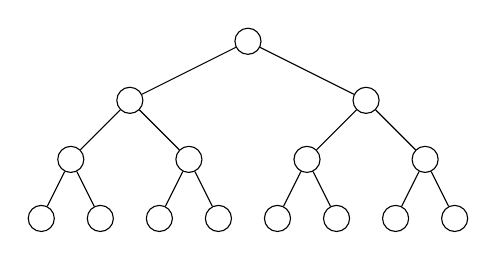
\begin{tikzpicture}
    [level distance=7.5mm,
      every node/.style={circle,draw},
      level 1/.style={sibling distance=30mm},
      level 2/.style={sibling distance=15mm},
      level 3/.style={sibling distance=7.5mm}]
    \node {}
      child {node {}
	child {node {}
	  child {node {}}
	  child {node {}}
	}
	child {node {}
	  child {node {}}
	  child {node {}}
	}
      }
      child {node {}
	child {node {}
	  child {node {}}
	  child {node {}}
	}
	child {node {}
	  child {node {}}
	  child {node {}}
	}
      };
  \end{tikzpicture}
\end{minipage}
\EP
Well, $S\subseteq U$, and usally $S\varsubsetneqq U$, so $|S|<|U|$, 
but we will assume that $S$ is not ``much'' smaller than $U$. That is, 
$u$ is polynomic in $n$ (not exponential), so $u\in poly(n)$, 
for instance: $u=n^5$. in that case, $log(n)$ is too much time. 
Assuming there's a solution that takes $O(log(log(u))$ time, 
may be such a solution is preferable to us. i.e. $n$ is very big, 
so: $u\in poly(n)\Longrightarrow log(u)=c\cdot{}log(n)\Longrightarrow log(n)=O(log(u))$, 
and the balanced binary tree solution is not good enough for us.

\BP
  a tree that is built above $U$:\\*
  \begin{minipage}{0.50725\textwidth}
    \medskip
    on one hand, we improved the solution suggested in Proposition~\ref{prop:VEB.I}, 
    such that \emph{successor} takes $O(log(u))$, but \emph{insert} also takes $O(log(u))$
    instead of the previously $O(1)$ time. This is because now we need to update all the 
    nodes while moving on the path towards the root. Searching for an element will be done 
    as follows: assume we are looking for the successor of $x$, then we start from $U[x]$,
    and move up untill we reach a vertex that is flaged with $1$ (of course, only in case
    that $x\in S$, and so $U[x]=0$, otherwise $x$'s parent will already be flages as $1$).
    if we reached a node from left, we will search the successor on the sub-tree hanging on 
    the right child, but if we reached the node from right, it is flaged $1$ only because 
    an element in the range that is smaller than $x$, and we should continue upwards on the 
    path. but, from now on, on every node we reached to from the left child, we have to 
    ``peek'' in the right child's flag, and check if it's $1$.
  \end{minipage}
  \begin{minipage}{0.45\textwidth}
    \setlength{\unitlength}{9mm}
    \begin{picture}(8.2,6)
    \linethickness{0.2mm}

    \put(0.2,0){\line(1,0){8}}
    \put(0.2,1){\line(1,0){8}}

    \put(0.2,0){\line(0,1){1}}
    \put(1.2,0){\line(0,1){1}}
    \put(2.2,0){\line(0,1){1}}
    \put(3.2,0){\line(0,1){1}}
    \put(4.2,0){\line(0,1){1}}
    \put(5.2,0){\line(0,1){1}}
    \put(6.2,0){\line(0,1){1}}
    \put(7.2,0){\line(0,1){1}}
    \put(8.2,0){\line(0,1){1}}

    \put(0.7,1.5){\circle*{0.25}}
    \put(1.7,1.5){\circle*{0.25}}
    \put(2.7,1.5){\circle*{0.25}}
    \put(3.7,1.5){\circle*{0.25}}
    \put(4.7,1.5){\circle*{0.25}}
    \put(5.7,1.5){\circle*{0.25}}
    \put(6.7,1.5){\circle*{0.25}}
    \put(7.7,1.5){\circle*{0.25}}

    \put(1.2,2){\circle*{0.25}}
    \put(3.2,2){\circle*{0.25}}
    \put(5.2,2){\circle*{0.25}}
    \put(7.2,2){\circle*{0.25}}

    \put(2.2,3){\circle*{0.25}}
    \put(6.2,3){\circle*{0.25}}

    \put(4.2,5){\circle*{0.25}}

    \put(0.7,1.5){\line(1,1){3.5}}
    \put(2.7,1.5){\line(1,1){0.5}}
    \put(4.7,1.5){\line(1,1){1.5}}
    \put(6.7,1.5){\line(1,1){0.5}}

    \put(1.7,1.5){\line(-1,1){0.5}}
    \put(3.7,1.5){\line(-1,1){1.5}}
    \put(5.7,1.5){\line(-1,1){0.5}}
    \put(7.7,1.5){\line(-1,1){3.5}}

    \put(0.6,0.4){0}
    \put(1.6,0.4){0}
    \put(2.6,0.4){1}
    \put(3.6,0.4){0}
    \put(4.6,0.4){0}
    \put(5.6,0.4){0}
    \put(6.6,0.4){1}
    \put(7.6,0.4){1}

    \put(4.1,5.25){1}
    \put(2.1,3.25){1}
    \put(6.1,3.25){1}
    \put(1.1,2.25){0}
    \put(3.1,2.25){1}
    \put(5.1,2.25){0}
    \put(7.1,2.25){1}
    \end{picture}
  \end{minipage}
\EP
Overall, \emph{successor} takes $O(log(u))$ time. we will try to improve:\\*
We can divide the vector into $\sqrt{u}$ segments the size of $\sqrt{u}$ each.
each of the segments, we can divide further into $\sqrt{\sqrt{u}}$ segments 
the size of $\sqrt{\sqrt{u}}$, and so on...\\*
\bigskip
\centering
\setlength{\unitlength}{6mm}
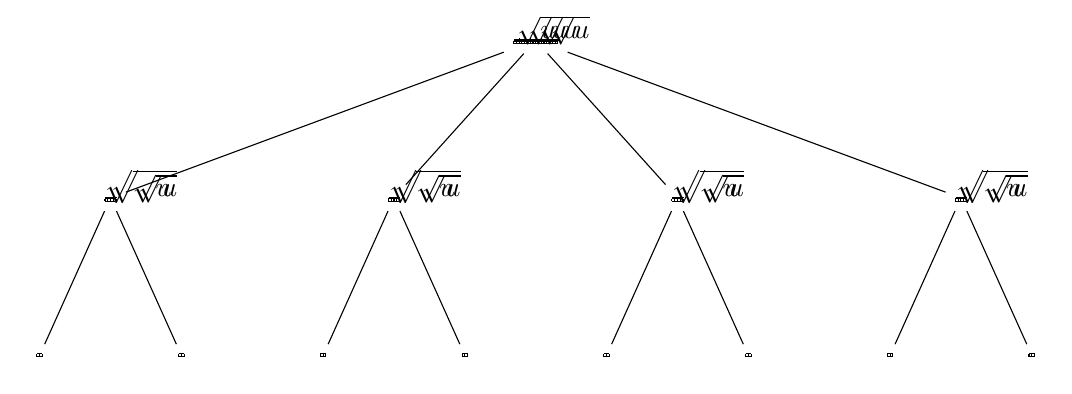
\begin{tikzpicture}
    [level distance=20mm,
      every node/.style={},
      level 1/.style={rectangle,sibling distance=36mm},
      level 2/.style={rectangle,sibling distance=18mm},
      level 3/.style={circle,draw,sibling distance=9mm}]
    \node {\begin{picture}(16,2.5)
	    \put(0,0){\line(1,0){16}}
	    \put(0,1){\line(1,0){16}}
	    \put(0,0){\line(0,1){1}}
	    \put(1,0){\line(0,1){1}}
	    \put(2,0){\line(0,1){1}}
	    \put(3,0){\line(0,1){1}}
	    \put(4,0){\line(0,1){1}}
	    \put(5,0){\line(0,1){1}}
	    \put(6,0){\line(0,1){1}}
	    \put(7,0){\line(0,1){1}}
	    \put(8,0){\line(0,1){1}}
	    \put(9,0){\line(0,1){1}}
	    \put(10,0){\line(0,1){1}}
	    \put(11,0){\line(0,1){1}}
	    \put(12,0){\line(0,1){1}}
	    \put(13,0){\line(0,1){1}}
	    \put(14,0){\line(0,1){1}}
	    \put(15,0){\line(0,1){1}}
	    \put(16,0){\line(0,1){1}}
	    \cbezier(0.1,1.25)(0.1,1.75)(2,1.25)(2,1.75)
	    \cbezier(3.9,1.25)(3.9,1.75)(2,1.25)(2,1.75)
	    \cbezier(4.1,1.25)(4.1,1.75)(6,1.25)(6,1.75)
	    \cbezier(7.9,1.25)(7.9,1.75)(6,1.25)(6,1.75)
	    \cbezier(8.1,1.25)(8.1,1.75)(10,1.25)(10,1.75)
	    \cbezier(11.9,1.25)(11.9,1.75)(10,1.25)(10,1.75)
	    \cbezier(12.1,1.25)(12.1,1.75)(14,1.25)(14,1.75)
	    \cbezier(15.9,1.25)(15.9,1.75)(14,1.25)(14,1.75)
	    \put(1.375,2){$\sqrt{u}$}
	    \put(5.375,2){$\sqrt{u}$}
	    \put(9.375,2){$\sqrt{u}$}
	    \put(13.375,2){$\sqrt{u}$}
	    \end{picture}}
      child {node {\begin{picture}(4,2.5)
                    \put(0,0){\line(1,0){4}}
                    \put(0,1){\line(1,0){4}}
                    \put(0,0){\line(0,1){1}}
                    \put(1,0){\line(0,1){1}}
                    \put(2,0){\line(0,1){1}}
                    \put(3,0){\line(0,1){1}}
                    \put(4,0){\line(0,1){1}}
		    \cbezier(0.1,1.25)(0.1,1.5)(1,1.25)(1,1.5)
		    \cbezier(1.9,1.25)(1.9,1.5)(1,1.25)(1,1.5)
		    \cbezier(2.1,1.25)(2.1,1.5)(3,1.25)(3,1.5)
		    \cbezier(3.9,1.25)(3.9,1.5)(3,1.25)(3,1.5)
		    \put(0,1.75){$\sqrt{\sqrt{u}}$}
		    \put(2,1.75){$\sqrt{\sqrt{u}}$}
                   \end{picture}}
	child {node {\begin{picture}(2,1)
                    \put(0,0){\line(1,0){2}}
                    \put(0,1){\line(1,0){2}}
                    \put(0,0){\line(0,1){1}}
                    \put(1,0){\line(0,1){1}}
                    \put(2,0){\line(0,1){1}}
                   \end{picture}}
	}
	child {node {\begin{picture}(2,1)
                    \put(0,0){\line(1,0){2}}
                    \put(0,1){\line(1,0){2}}
                    \put(0,0){\line(0,1){1}}
                    \put(1,0){\line(0,1){1}}
                    \put(2,0){\line(0,1){1}}
                   \end{picture}}
	}
      }
      child {node {\begin{picture}(4,2.5)
                    \put(0,0){\line(1,0){4}}
                    \put(0,1){\line(1,0){4}}
                    \put(0,0){\line(0,1){1}}
                    \put(1,0){\line(0,1){1}}
                    \put(2,0){\line(0,1){1}}
                    \put(3,0){\line(0,1){1}}
                    \put(4,0){\line(0,1){1}}
		    \cbezier(0.1,1.25)(0.1,1.5)(1,1.25)(1,1.5)
		    \cbezier(1.9,1.25)(1.9,1.5)(1,1.25)(1,1.5)
		    \cbezier(2.1,1.25)(2.1,1.5)(3,1.25)(3,1.5)
		    \cbezier(3.9,1.25)(3.9,1.5)(3,1.25)(3,1.5)
		    \put(0,1.75){$\sqrt{\sqrt{u}}$}
		    \put(2,1.75){$\sqrt{\sqrt{u}}$}
                   \end{picture}}
	child {node {\begin{picture}(2,1)
                    \put(0,0){\line(1,0){2}}
                    \put(0,1){\line(1,0){2}}
                    \put(0,0){\line(0,1){1}}
                    \put(1,0){\line(0,1){1}}
                    \put(2,0){\line(0,1){1}}
                   \end{picture}}
	}
	child {node {\begin{picture}(2,1)
                    \put(0,0){\line(1,0){2}}
                    \put(0,1){\line(1,0){2}}
                    \put(0,0){\line(0,1){1}}
                    \put(1,0){\line(0,1){1}}
                    \put(2,0){\line(0,1){1}}
                   \end{picture}}
	}
      }
      child {node {\begin{picture}(4,2.5)
                    \put(0,0){\line(1,0){4}}
                    \put(0,1){\line(1,0){4}}
                    \put(0,0){\line(0,1){1}}
                    \put(1,0){\line(0,1){1}}
                    \put(2,0){\line(0,1){1}}
                    \put(3,0){\line(0,1){1}}
                    \put(4,0){\line(0,1){1}}
		    \cbezier(0.1,1.25)(0.1,1.5)(1,1.25)(1,1.5)
		    \cbezier(1.9,1.25)(1.9,1.5)(1,1.25)(1,1.5)
		    \cbezier(2.1,1.25)(2.1,1.5)(3,1.25)(3,1.5)
		    \cbezier(3.9,1.25)(3.9,1.5)(3,1.25)(3,1.5)
		    \put(0,1.75){$\sqrt{\sqrt{u}}$}
		    \put(2,1.75){$\sqrt{\sqrt{u}}$}
                   \end{picture}}
	child {node {\begin{picture}(2,1)
                    \put(0,0){\line(1,0){2}}
                    \put(0,1){\line(1,0){2}}
                    \put(0,0){\line(0,1){1}}
                    \put(1,0){\line(0,1){1}}
                    \put(2,0){\line(0,1){1}}
                   \end{picture}}
	}
	child {node {\begin{picture}(2,1)
                    \put(0,0){\line(1,0){2}}
                    \put(0,1){\line(1,0){2}}
                    \put(0,0){\line(0,1){1}}
                    \put(1,0){\line(0,1){1}}
                    \put(2,0){\line(0,1){1}}
                   \end{picture}}
	}
      }
      child {node {\begin{picture}(4,2.5)
                    \put(0,0){\line(1,0){4}}
                    \put(0,1){\line(1,0){4}}
                    \put(0,0){\line(0,1){1}}
                    \put(1,0){\line(0,1){1}}
                    \put(2,0){\line(0,1){1}}
                    \put(3,0){\line(0,1){1}}
                    \put(4,0){\line(0,1){1}}
		    \cbezier(0.1,1.25)(0.1,1.5)(1,1.25)(1,1.5)
		    \cbezier(1.9,1.25)(1.9,1.5)(1,1.25)(1,1.5)
		    \cbezier(2.1,1.25)(2.1,1.5)(3,1.25)(3,1.5)
		    \cbezier(3.9,1.25)(3.9,1.5)(3,1.25)(3,1.5)
		    \put(0,1.75){$\sqrt{\sqrt{u}}$}
		    \put(2,1.75){$\sqrt{\sqrt{u}}$}
                   \end{picture}}
	child {node {\begin{picture}(2,1)
                    \put(0,0){\line(1,0){2}}
                    \put(0,1){\line(1,0){2}}
                    \put(0,0){\line(0,1){1}}
                    \put(1,0){\line(0,1){1}}
                    \put(2,0){\line(0,1){1}}
                   \end{picture}}
	}
	child {node {\begin{picture}(2,1)
                    \put(0,0){\line(1,0){2}}
                    \put(0,1){\line(1,0){2}}
                    \put(0,0){\line(0,1){1}}
                    \put(1,0){\line(0,1){1}}
                    \put(2,0){\line(0,1){1}}
                   \end{picture}}
	}
      };
  \end{tikzpicture}
\setlength{\unitlength}{10mm}
\flushleft
\begin{align*}
T(u) &= \text{time to do ``something'' in a structure of size $u$} \\
T(u) &= T(\sqrt{u}) + 1 \\
T(2) &= 1 \\
T(u) &= T(u^{\frac{1}{2}}) + 1 = T(u^{\frac{1}{2^2}}) + 2 = T(u^{\frac{1}{2^3}}) + 3 = \ldots \\
&\Longrightarrow T(u^{\frac{1}{2^i}}) + i \\
u^{\frac{1}{2^i}} &= 2 \\
&\iff \big(2^{log(u)}\big)^{\frac{1}{2^i}} = 2 
 \iff log(u)\cdot{}\frac{1}{2^i} = 1 
 \iff 2^i = log(u) \\
&\iff i = log(log(u))
\end{align*}
Actually, we can look at the structure ``recursively'', 
that is, in the lowest level there's $\sqrt{u}$ structures, 
each the size of $\sqrt{u}$, 
in the level above, there's $\sqrt{\sqrt{u}}$ structures, 
each the size of $\sqrt{\sqrt{u}}$.\\*
well, now we have $\sqrt{t}$ arrays at each level, 
where's $t$ is the number of arrays in the preceding level.\\
%
%
% NOTE TO SELF: image here?
%
%
\BN
\begin{align*}
  sub[0] \text{ } &\text{- the structure (array) of the first $\sqrt{u}$ elements} \\
  sub[1] \text{ } &\text{- the structure (array) of the next $\sqrt{u}$ elements} \\
          &\vdots  \\
sub[u-1] \text{ } &\text{- the structure (array) of the last $\sqrt{u}$ elements} \\
\end{align*}
\EN
In general, $sub[i]$ is the structure of the $\sqrt{u}$ elements: 
$i\cdot\sqrt{u},\ldots{},(i+1)\cdot\sqrt{u}-1$\\*
well, how would we implement $succ(x)$ or $pred(x)$ algorithms?\\*
\BP
we can look at a higher level, and check if the representative is $0$, 
if so, we should continue the scan untill the end of the structure, 
if all were zeros, we should continue to the next structure, and so on.
if we found $1$, we should go down to it's sub-set, 
where it is guaranteed to have a \emph{successor\slash{}predecessor}.\\
\textbf{Time:} $O(\sqrt{u})$
\EP
Still not good enough. we can look at the binary 
representation of an element (number) $x$ in our structure, 
when we assume (for convenience) that $u=2^k,k\in \mathbb{N}$.
if so, the length of $x$'s representation is of size $log(u)$.
we will divide the representation of $x$ in half, and notate:
\BN
\item \setlength{\unitlength}{10mm}
\begin{picture}(10,3.25)
  \linethickness{0.2mm}
  \put(0,2){\line(1,0){10}}
  \put(0,3){\line(1,0){10}}
  \put(0,2){\line(0,1){1}}
  \put(1,2){\line(0,1){1}}
  \put(5,2){\line(0,1){1}}
  \put(9,2){\line(0,1){1}}
  \put(10,2){\line(0,1){1}}
  \put(0.4,1.6){$0$}
  \put(9.1,1.6){$u-1$}
  \cbezier(0.1,1.4)(0.1,0.65)(2.5,1.4)(2.5,0.65)
  \cbezier(4.9,1.4)(4.9,0.65)(2.5,1.4)(2.5,0.65)
  \cbezier(5.1,1.4)(5.1,0.65)(7.5,1.4)(7.5,0.65)
  \cbezier(9.9,1.4)(9.9,0.65)(7.5,1.4)(7.5,0.65)
  \put(2,0){$high(x)$}
  \put(7,0){$low(x)$}
\end{picture}
\EN
\bigskip
Each part of the representation, is the length of $\frac{1}{2}\cdot{}log(u)$, 
and the number of elements we can represent with $\frac{1}{2}\cdot{}log(u)$ bits, is: 
$2^{\frac{1}{2}\cdot{}log(u)}=(2^{log(u)})^{\frac{1}{2}}=u^{\frac{1}{2}}=\sqrt{u}$.\\*
in general, according to our notation: 
$$x=high(x)\cdot{2^{\frac{log(u)}{2}}}+low(x)$$
So, if we want to find the set\slash{}array $sub[i]$ of $x$, 
we can compute: $x\in{sub[high(x)}]$. 
we can see that all the first $\sqrt{u}$ elements has the same $high(x)$:\\
\bigskip
\setlength{\unitlength}{5mm}
\begin{picture}(21,12)
  \linethickness{0.2mm}
  \put(9,2){\line(1,0){12}}
  \put(9,3){\line(1,0){12}}
  \put(9,4){\line(1,0){12}}
  \put(9,6){\line(1,0){12}}
  \put(9,7){\line(1,0){12}}
  \put(9,8){\line(1,0){12}}
  \put(9,10){\line(1,0){12}}
  \put(9,11){\line(1,0){12}}
  \put(9,12){\line(1,0){12}}
  \put(9,2){\line(0,1){10}}
  \put(15,2){\color[rgb]{0.75,0.75,0.75}{\line(0,1){10}}}
  \put(21,2){\line(0,1){10}}
  \put(9.25,11.25){$0$}
  \put(10.25,11.25){$0$}
  \put(14.25,11.25){$0$}
  \put(15.25,11.25){$0$}
  \put(19.25,11.25){$0$}
  \put(20.25,11.25){$0$}
  \put(12,11.3){$\cdots$}
  \put(17,11.3){$\cdots$}
  \put(9.25,10.25){$0$}
  \put(10.25,10.25){$0$}
  \put(14.25,10.25){$0$}
  \put(15.25,10.25){$0$}
  \put(19.25,10.25){$0$}
  \put(20.25,10.25){$1$}
  \put(12,10.3){$\cdots$}
  \put(17,10.3){$\cdots$}
  \put(9.25,7.25){$0$}
  \put(10.25,7.25){$0$}
  \put(14.25,7.25){$0$}
  \put(15.25,7.25){$1$}
  \put(19.25,7.25){$1$}
  \put(20.25,7.25){$1$}
  \put(12,7.3){$\cdots$}
  \put(17,7.3){$\cdots$}
  \put(9.25,6.25){$0$}
  \put(10.25,6.25){$0$}
  \put(14.25,6.25){$1$}
  \put(15.25,6.25){$0$}
  \put(19.25,6.25){$0$}
  \put(20.25,6.25){$0$}
  \put(12,6.3){$\cdots$}
  \put(17,6.3){$\cdots$}
  \put(9.25,3.25){$0$}
  \put(10.25,3.25){$0$}
  \put(14.25,3.25){$1$}
  \put(15.25,3.25){$1$}
  \put(19.25,3.25){$1$}
  \put(20.25,3.25){$0$}
  \put(12,3.3){$\cdots$}
  \put(17,3.3){$\cdots$}
  \put(9.25,2.25){$0$}
  \put(10.25,2.25){$0$}
  \put(14.25,2.25){$1$}
  \put(15.25,2.25){$1$}
  \put(19.25,2.25){$1$}
  \put(20.25,2.25){$1$}
  \put(12,2.3){$\cdots$}
  \put(17,2.3){$\cdots$}
  \put(12.333,8.667){$\vdots$}
  \put(17.333,8.667){$\vdots$}
  \put(12.333,4.667){$\vdots$}
  \put(17.333,4.667){$\vdots$}
  \cbezier(8.433,11.9)(7.667,11.9)(8.433,9.5)(7.667,9.5)
  \cbezier(8.433,7.1)(7.667,7.1)(8.433,9.5)(7.667,9.5)
  \cbezier(8.433,6.9)(7.667,6.9)(8.433,4.5)(7.667,4.5)
  \cbezier(8.433,2.1)(7.667,2.1)(8.433,4.5)(7.667,4.5)
  \put(0,9.3){$\text{the first $\sqrt{u}$ elements}$}
  \put(0,4.3){$\text{the next $\sqrt{u}$ elements}$}
  \put(3.667,0){$\vdots$}
  \put(15,0){$\vdots$}
\end{picture}
\setlength{\unitlength}{10mm}
\medskip
\\Well then, $high(x)$ determines in which ``sub-group'' $x$ is found, 
and $low(x)$ determines where exactly in the group it is found. if $S$, 
our structure, is of size $|S|$:
$sub[S][0],sub[S][1],sub[S][2],\ldots{},sub[S][\sqrt{u}-1]$, 
we would probably want to store an extra bit array the size of $\sqrt{u}$ 
to check quickly if there's an element in the array $sub[S][i]$. 
that is (we will call this extra array: $summary[S]$): 
$\big((summary \ AND \ 2^i) == 2^i\big)\Longrightarrow \exists \ x\in sub[S][i]$\\*
so the size of $summary[S]$ is $\sqrt{|S|}$, and it help us determine if $sub[S][i]$ 
is empty or not, according to the $i$ bit. so how do we perform $insert(x)$?
\BAL
insert(x,S)
\begin{itemize}
 \item[1.] flag $\gets$ isEmpty($sub[S][high(x)]$)
 \item[2.] $insert(low(x),sub[S][high(x)])$
 \item[3.] if(flag)
 \begin{itemize}
  \item[3.1.] then $insert(high(x),summary[S])$
 \end{itemize}
\end{itemize}
\EAL
So, how much time does this takes? (assuming the size of the structure is $u$):
$$T(u)=2T(\sqrt{u})+1=2^2\cdot{T(u^{\frac{1}{2^2}})}+2+1=
2^3\cdot{T(u^{\frac{1}{2^3}})}+4+2+1=\ldots{}=
2^i\cdot{T(u^{\frac{1}{2^i}})}+\sum_{j=0}^{i-1}2^j=log(u)$$
Not so good. we are back to $O(log(u))$ time.\footnotemark \\*
\footnotetext{$|U|>|S|\Longrightarrow{u>n}\Longrightarrow{log(u)>log(n)}$, 
so we better off with a ``regular'' balanced tree (AVL\slash{Red-Black}\slash{etc'...})}
This happens because we have 2 recursive calls for $insert$.\\
\newpage
let's check $successor$ also:
\BAL
succ(x,S)
  \item[1.] $j\gets{succ\big(low(x),sub[S][high(x)]\big)}$
  \item[2.] if $j<\infty$
  \begin{itemize}
    \item[2.1.] return $high(x)\cdot{\sqrt{|S|}}+j$
  \end{itemize}
  \item[3.] $i\gets{succ\big(high(x)+1,summary[S]\big)}$
  \item[4.] if $i=\infty$
  \begin{itemize}
    \item[4.1.] return $\infty$
  \end{itemize}
  \item[5.] $j\gets{succ\big(0,sub[S][i]\big)}$
  \item[6.] return $i\cdot{\sqrt{|S|}+j}$
\EAL
Well, this suggested algorithm takes: 
$T(u)=3\cdot{T(\sqrt{u})+1}\Longrightarrow{O\big(T(u)\big)\gg{O\big(log(u)\big)}}$ 
which is even worse than what we had on $insert$. the reason for this is that we have 3 
recursive calls for $succ$, which we invoke because we want to find the successor element 
when were in a structure, that queried for an element that is greater than the max element 
in this structure. this means we need to search the next structure. if we had known this 
in advanced, it would have saved us a lot of time. we will try to improve:
\BP
we can add to each structure, an extra 2 elements indicating the 
minimum \& maximum elements in the structure.\\
\begin{picture}(12,4.25)
  \put(0,2.9){$S=\text{ \ \ \ }summary,sub[S][0],\ldots{},sub[S][\sqrt{|S|}-1],min,max$}
  \put(1,2.5){\line(0,1){1}}
  \put(10.375,2.5){\line(0,1){1}}
  \put(1,2.5){\line(1,0){9.375}}
  \put(1,3.5){\line(1,0){9.375}}
  \put(4,2.7){\vector(0,-1){1}}
  \put(3.2,0.7){\line(0,1){1}}
  \put(8,0.7){\line(0,1){1}}
  \put(3.2,0.7){\line(1,0){4.8}}
  \put(3.2,1.7){\line(1,0){4.8}}
  \put(1,1.1){$sub[S][0]=\text{ \ \ \ }summary,\ldots{},min,max\text{ \ \ \ }\cdots$}
\end{picture}
\EP
Now, with the modified structure, how can we find the \emph{successor} of some element $x$?
\BAL
succ(x,S)
  \item[1.] if $low(x) < max\big(sub[S][high(x)]\big)$
  \begin{itemize}
    \item[1.1.] $j\gets{succ\big(low(x),sub[S][high(x)]\big)}$
    \item[1.2.] return $high(x)\cdot{\sqrt{|S|}}+j$
  \end{itemize}
  \item[2.] else
  \begin{itemize}
    \item[2.1.] $i\gets{succ\big(high(x)+1,summary[S]\big)}$
    \item[2.2.] if $i=\infty$
    \begin{itemize}
      \item[2.2.1] return $\infty$ 
    \end{itemize}
    \item[2.3.] return $i\cdot{\sqrt{|S|}}+min\big(sub[S][i]\big)$
  \end{itemize}
\EAL
\newpage
So now, we only have 1 recursive call, so the overall time for \emph{successor} is 
$T(u)=T(\sqrt{u})+1=\ldots{=O\Big(log\big(log(n)\big)\Big)}$. but we ignored \emph{insert},
which will now need more updates of the new data ($min,max$) we entered,
so, have we worsen the problem for \emph{insert}?.

Well, not only that we hav'nt made it worse, we actually made it better!
we now only need to update $summary$ once, and we don't realy need to update $min,max$ 
every time. we will update only when we first put an element in, and from now on, 
we can simply switch our newly inserted element, in case it is bigger (smaller) than 
the $max$ ($min$), and continue with the recursive insertion with the old $max$ ($min$) element.
let's see how the new algorithm will work:
\BAL
insert(x,S)
\begin{itemize}
  \item[1.] if $x<min[S]$
  \begin{itemize}
    \item[1.1.] switch$\big(min[S],x\big)$
  \end{itemize}
  \item[2.] if $isEmpty\big(sub[S][high(x)]\big)$
  \begin{itemize}
    \item[2.1.] $min\big(sub[S][high(x)]\big)\gets{low(x)}$
    \item[2.2.] $insert\big(high(x),summary[S]\big)$
  \end{itemize}
  \item[3.] else
  \begin{itemize}
    \item[3.1.] $insert\big(low(x),sub[S][high(x)]\big)$
  \end{itemize}
  \item[4.] if $x>max[S]$
  \begin{itemize}
   \item[4.1.] $max[S]\gets{x}$
  \end{itemize}
\end{itemize}
\EAL
now, \emph{insert} has only 1 recursive call like \emph{successor}, and so, 
it takes $O\Big(log\big(log(n)\big)\Big)$ as well. so overall, 
we improved the time complexity:
  \item[\textbf{Successor:}] $O\Big(log\big(log(u)\big)\Big)$
  \item[\textbf{Insert: {} {} }] $O\Big(log\big(log(u)\big)\Big)$

\medskip
the space complexity is:
  \item[\textbf{Space: {} {} }] $O(u)$

\bigskip
these are the final results.\\
and as the title states, this data structure is 
named after it's inventor: \emph{Van-Emde Boas}
\newpage

\section{X-Fast Trie}
we allready saw previously the \emph{Van-Emde Boas} trees(~\ref{subsection:VEB}),
and the space complexity for this data structure was:
$S(u)=\sqrt{u}S(\sqrt{u})+\sqrt{u}\textcolor[rgb]{1,0,0}{\footnotemark}$, 
\footnotetext{$\sqrt{u}$ in every level for the summary.}
the ``height'' of the structure is:
$H(u)=H(\sqrt{u})+1=log(log(u))$, so the total space capacity is:
%\begin{equation*}
\begin{align*}
S(u)\nonumber &=\sqrt{u}\cdot{}S(\sqrt{u})+\sqrt{u}=
\sqrt{u}+\sqrt{u}\sqrt{\sqrt{u}}+\sqrt{u}\sqrt{\sqrt{u}}\cdot{}S(\sqrt{\sqrt{u}})=
\ldots{}\nonumber \\ &=
u^{\frac{1}{2}+\frac{1}{4}+\frac{1}{8}+\ldots{}+\frac{1}{2^{log(log(u))}}}
+\sum_{i=0}^{2^{log(log(u))}}u^{\frac{1}{2^i}} =
u^{1-\frac{1}{log(u)}}+\sum_{i=0}^{log(u)}u^{\frac{1}{2^i}}
\approx{}O(u)\nonumber
\end{align*}
%\end{equation*}
so the Van-Emde Boas data structure can support the actions 
\emph{insert,delete,successor,predecessor} in $O\Big(log\big(log(u)\big)\Big)$
but the space complexity is linear in $u$. can it be improved?\\*
\medskip
$S=\{x_1,x_2,\ldots{},x_n\}, S\subseteq U$\\*
\begin{picture}(6.5,5.5)
\put(0,1.75){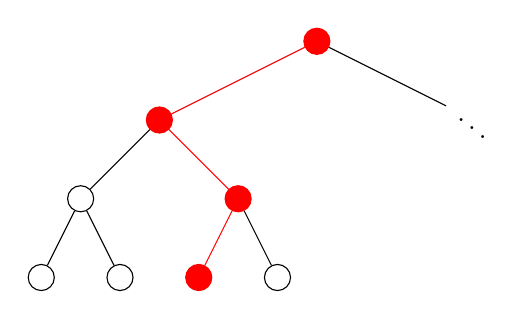
\begin{tikzpicture}
  [level distance=10mm,
    %every node/.style={circle,draw},
    level 1/.style={sibling distance=40mm},
    level 2/.style={sibling distance=20mm},
    level 3/.style={sibling distance=10mm}]
  \node[style={circle,fill,draw},color=red] {}
    child[red] {node[style={circle,fill,draw}] {}
      child[black] {node[style={circle,draw}] {}
	child {node[style={circle,draw}] {}}
	child {node[style={circle,draw}] {}}
      }
      child {node[style={circle,fill,draw}] {}
	child {node[style={circle,fill,draw}] {}}
	child[black] {node[style={circle,draw}] {}}
      }
    }
    child {node {$\ddots{}$}
    };
\end{tikzpicture}}
\put(2.4,0.9){$x$}
\put(0,0.5){\line(1,0){8}}
\put(0,1.5){\line(1,0){8}}
\put(0,0.5){\line(0,1){1}}
\put(1,0.5){\line(0,1){1}}
\put(2,0.5){\line(0,1){1}}
\put(3,0.5){\line(0,1){1}}
\put(4,0.5){\line(0,1){1}}
\put(8,0.5){\line(0,1){1}}

\put(0.4,0){$0$}
\put(1.4,0){$1$}
\put(2.4,0){\textcolor[rgb]{1,0,0}{$\textbf{2}$}}
\put(3.4,0){$3$}
\put(4.4,0){$\cdots{}$}
\end{picture}

actually, we don't realy need edges. in the above example, 
$x=2 \Longrightarrow \text{the binary representation of x is: }010$, 
and the path from $x$ upwards is: \emph{left$\to{}$right$\to{}$left}, 
which confronts to $0\to{}1\to{}0$. in general, 
when looking into the bitwise representation of an element $x$, 
we can ``travel'' it's path to the root by starting from the \emph{LSB}, 
and moving towards the \emph{MSB}, while turning right whenever we encounter $0$, 
and turning left when we encounter $1$.
\newpage

\section{Y-Fast Trie}
some text to be inserted here
\newpage

\section{Cukoo Hashing}
some text to be inserted here
\newpage

\chapter{Data Structures for Strings}
\section{Pattern Matching}
\subsection{Suffix Tree}
some text to be inserted here
\newpage

\subsection{Suffix Array}
some text to be inserted here
\newpage

\section{LCP - Longest Common Prefix}
\subsection{Kasai's Algorithm}
some text to be inserted here
\newpage

\section{RMQ - Range Minimum Query}
\subsection{Cartesian Tree}
some text to be inserted here
\newpage

\section{Misc}
\subsection{General Problems}
LCA,Palindrom,K-mistakes\ldots{}
\newpage

\subsection{Karkaihner \& Sanders Algorithm}
some text to be inserted here
\newpage

\chapter{Trees}
\section{Tree Decomposition}
\subsection{Centroid Path Decomposition}
some text to be inserted here
\newpage

\subsection{Heavy Path Decomposition}
some text to be inserted here
\newpage

\chapter{Special Properties for Data Structures}
\section{Persistent Data Structures}
\newpage

\section{Succint Data Structures}


\bibliography{AdvancedDS}
\bibliographystyle{alpha}
\addcontentsline{toc}{chapter}{Bibliography}

\end{document}